
\begin{question}
It is generally accepted that a population's proportion is 0.393.
However, you think that maybe the population proportion is not 0.393, so
you decide to run a two-tail hypothesis test with a significance level
of 0.02 with a sample size of 4000.

Then, when you collect the random sample, you find its proportion is
0.413. Do you reject or retain the null hypothesis?
\begin{answerlist}
  \item Determine the \(p\)-value.
  \item Decide whether we reject or retain the null hypothesis.
\end{answerlist}
\end{question}

\begin{solution}
State the hypotheses. \[H_0: ~~ p = 0.393 \]
\[H_\text{A}: ~~ p \ne 0.393\] Determine the standard error.
\[SE = \sqrt{\frac{p_0(1-p_0)}{n}} = \sqrt{\frac{0.393(1-0.393)}{4000}} = 0.00772 \]
Determine a \(z\) score. For simplicity, we ignore the continuity
correction.
\[z = \frac{\hat{p}-p_0}{SE} = \frac{0.413-0.393}{0.00772} = 2.59 \] The
\(p\)-value is a two-tail area.

\begin{figure}[htbp]
\centering
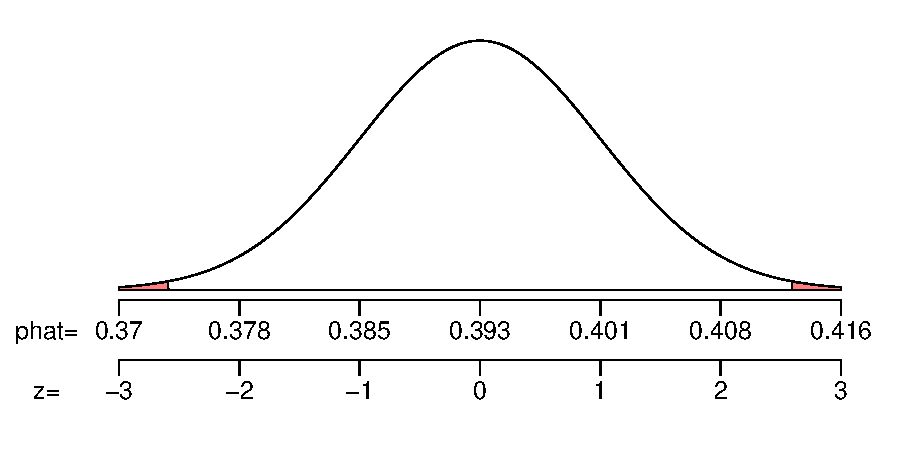
\includegraphics{p_single_test_twotail-1.pdf}
\caption{}
\end{figure}

To determine that two-tail area, we use the z table.
\[\text{Pr}\left(\hat{P} > 0.413\right) ~=~ 2\cdot \Phi(-2.59) ~=~ 0.0096 \]
In other words: \[p\text{-value} = 0.0096\] Compare \(p\)-value to
\(\alpha\) (which is 0.02). \[p\text{-value} < \alpha \] Make the
conclusion: we reject the null hypothesis.
\begin{answerlist}
  \item The \(p\)-value is 0.0096
  \item We reject the null hypothesis.
\end{answerlist}
\end{solution}

